\let\textcircled=\pgftextcircled
\chapter{Multi-variable Emulation}
\label{chap:mv}

\section{Introduction}
\label{mv:intro}

ML has been shown to be effective in emulating high-resolution climate model even for a highly variable and stochastic setting like UK precipitation.
However, it is often important to have coherent samples of more than one variable. For example, heat stress may involve air temp, humidity and wind speed \cite{Blazejczyk2012UTCIcomparison}. Indices have been created to simplify complex joint distributions into a single value. This allows a method for evaluating joint samples from a multivariate emulator - as well as modelling the marginal distributions of each variable and capturing some elements of the joint distribution, ideally the emulator should be able to recreate the same distribution of a compound index.
These indicies also allow us to focus on high impact events - for example it is more important to capture the distribution of stressfully hot days rather than small variations on more temperate days.

\section{Method}
\label{mv:method}

\subsection{Data}

\subsubsection{Target Variables}

\begin{itemize}
    \item Temp at 1.5m
    \item relhum at 1.5m
    \item precip
\end{itemize}

\subsubsection{Indices}

I start with the \acrfull{swbgt} index. This is an approximation of wet bulb globe temperature that can be calculated with only relative humidity and air temperature \parencite[e.g][]{Blazejczyk2012UTCIcomparison, zhao2015heatstresscmip5, buzan2015heatstress} and used by the Australian Bureau of Meteorology (\url{http://www.bom.gov.au/info/thermal_stress/}, 16 March 2011).
Although there may be issues with this simplification \parencite{kong2022wbgtapproxissues} that get worse in a changing climate but these are more pronounced in locations with more extreme heat and humidity the UK \parencite{qiu2024swbgtbias}. \textcite{kong2022wbgtapproxissues} suggest ESI as an alternative (though the true preference would be to avoid approximations and use a recent WBGT calculation that takes into account wind speed and radiation).


\section{results}
\label{mv:results}

\begin{figure}[ht]
	\centering
	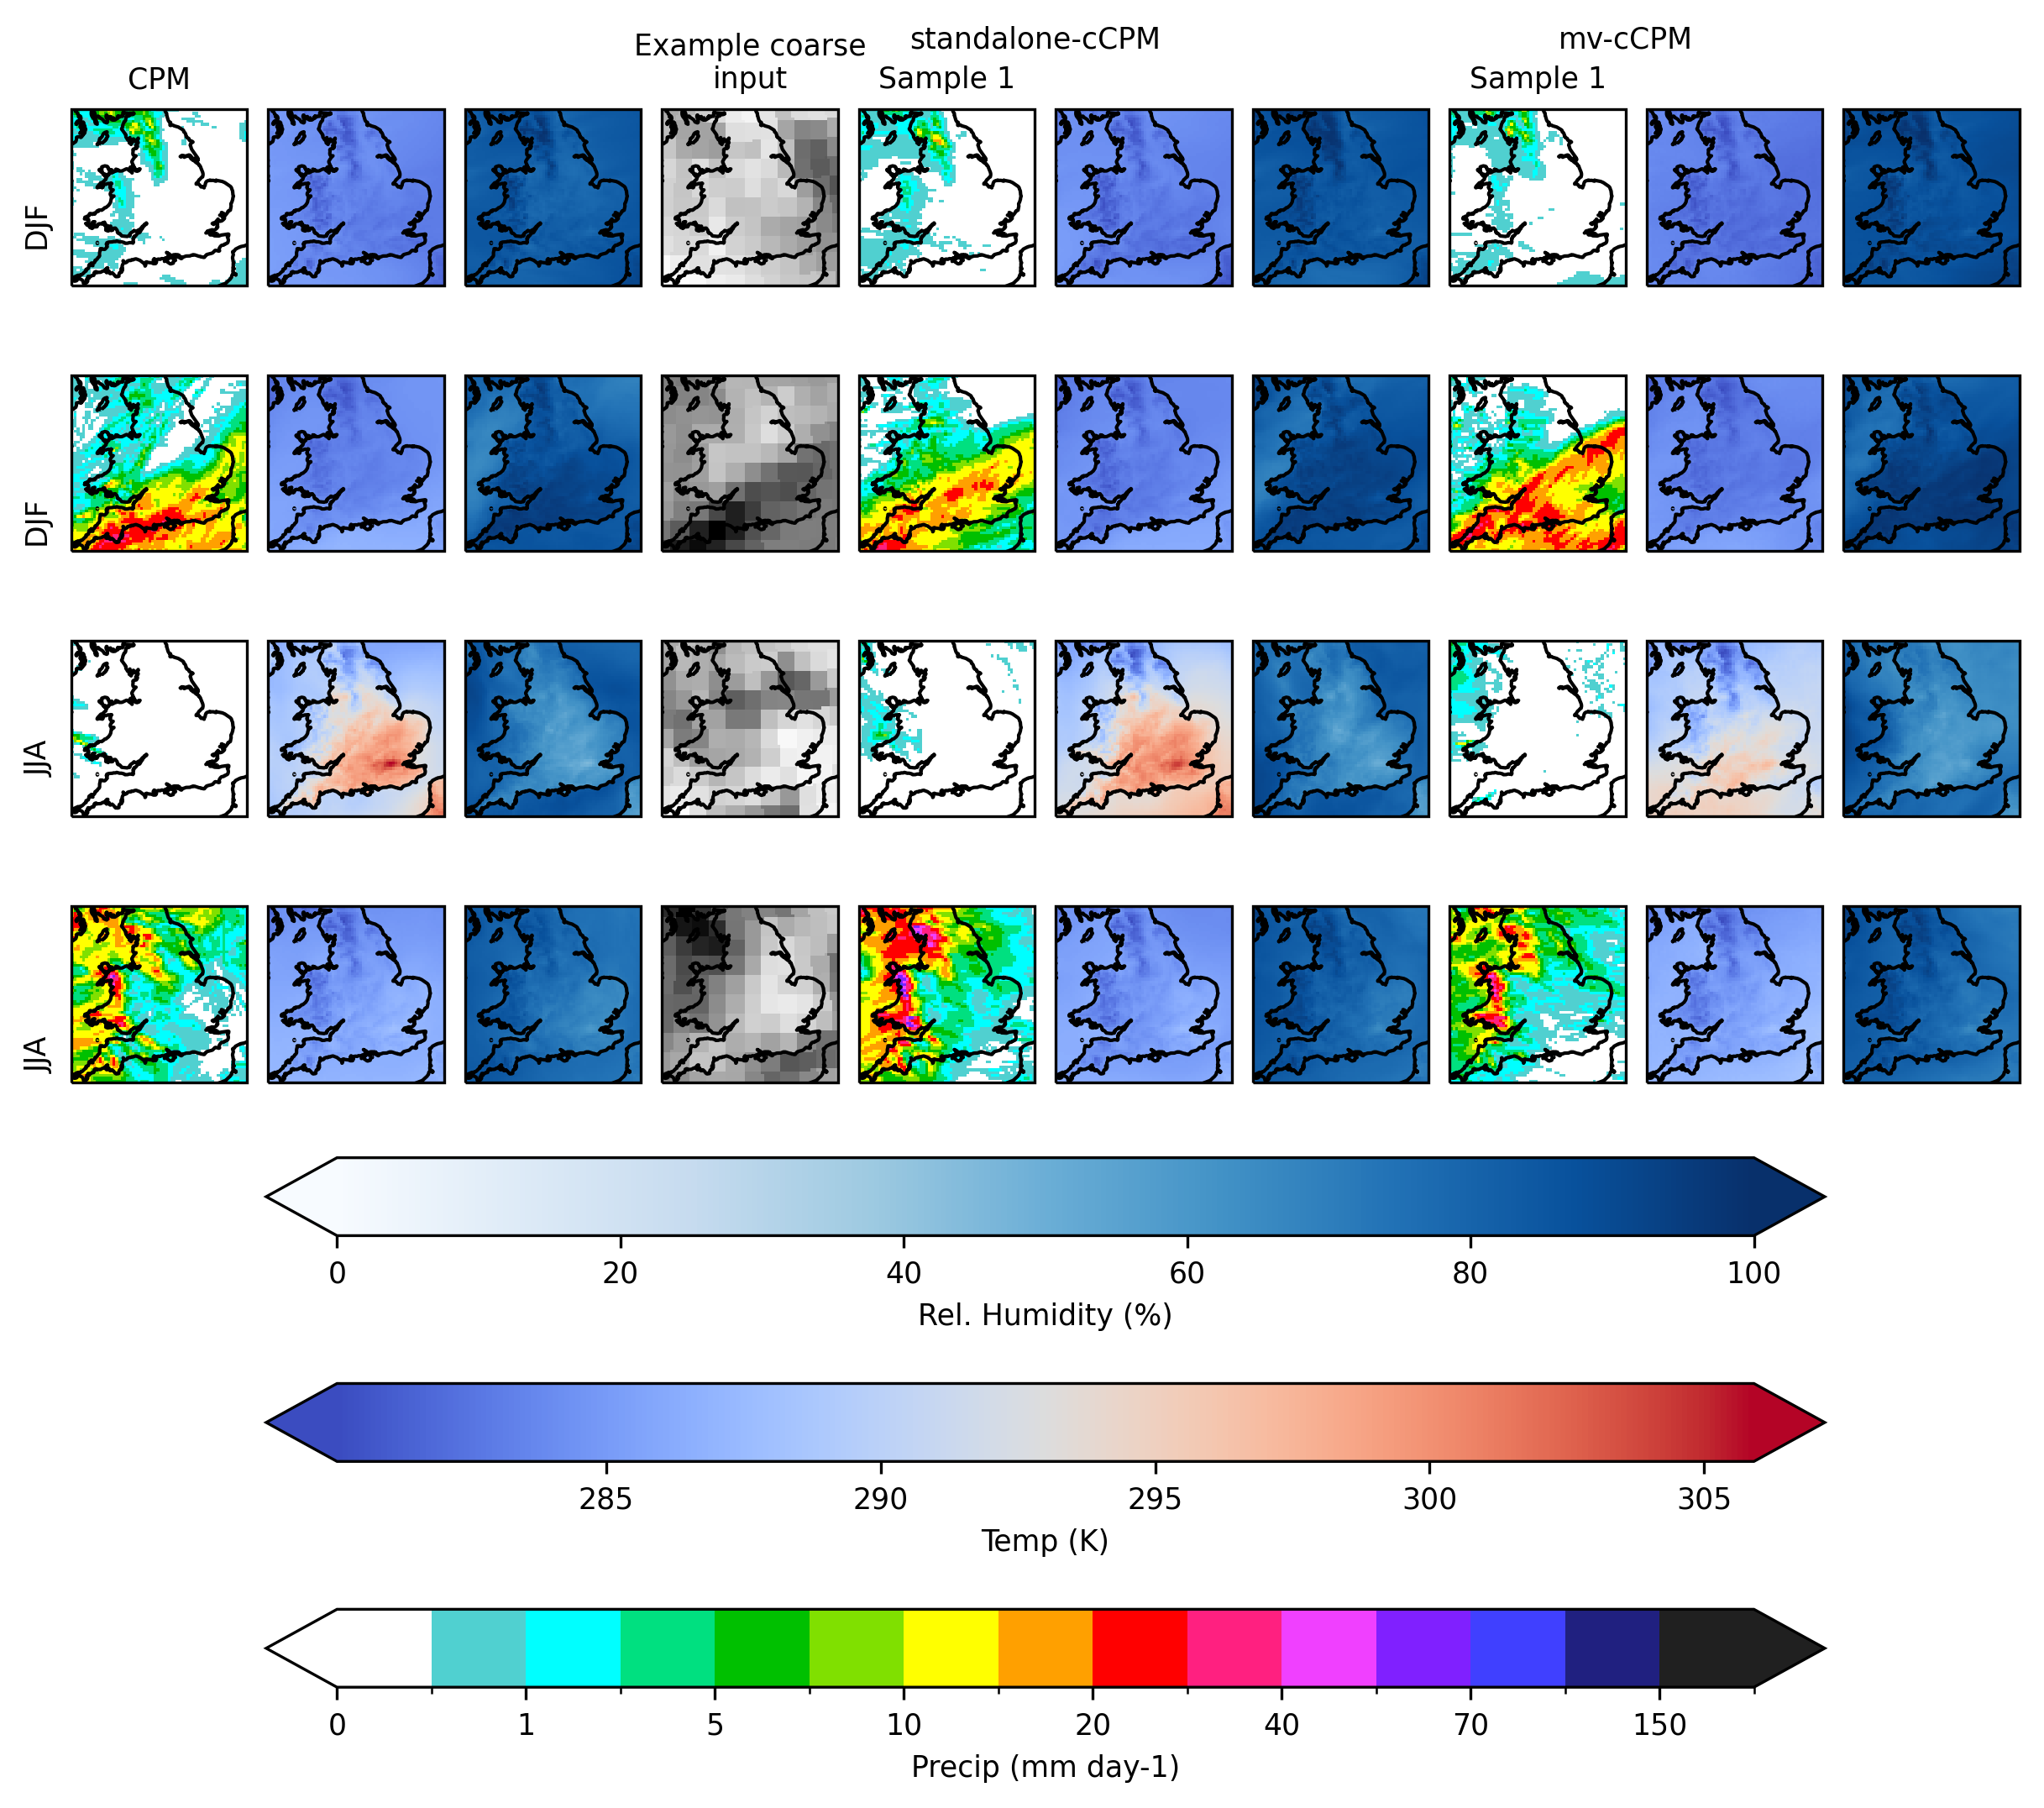
\includegraphics[height=0.35\textheight]{chapters/figures/5_mv/mv-samples.png}
	\caption{Multivariate samples from a multivariate model and a combination of samples from univariate models (one for each variable). For the former, a single emulator produces samples of all variables in one go. In the latter case, samples of each variable are randomly paired.}
	\label{fig:mv-samples}
\end{figure}

I compare stand-alone univariate models for three variables (hurs, tas and pr) against a single multivariate model that models all three. I would expect on many univariate analyses the univariate model would out-perform the multivariate model but would not do so well for any analysis that uses the joint distribution of more than one of these variables.
However, I find for the univarate marginal distribution, the multivariate does better.
This could be because:
\begin{itemize}
    \item the joint distribution of the target variables contains information that constrains them even if it is a more complex distribution to model
    \item the univariate models are overfitting
    \item something about the model is tailored to heavily to precipitation
    \item
\end{itemize}

Actually the diffusion model should be powerful enough that it can learn the multivariate version no worse than a stand-alone.